%==============================================================================
% Cloud Computing (SE-490) - Complex Engineering Activity - Technical Report
% PDF Toolkit: Three-Tier Web Application on AWS
% Title page + 6 pages (page limit of the CEA statement).
%==============================================================================
\documentclass[11pt,a4paper]{article}

\usepackage[a4paper,top=0.65in,bottom=0.7in,left=0.7in,right=0.7in,headsep=6pt,footskip=16pt]{geometry}
\usepackage{times}
\usepackage[T1]{fontenc}
\usepackage[utf8]{inputenc}
\usepackage{graphicx}
\usepackage{xcolor}
\usepackage{booktabs}
\usepackage{array}
\usepackage{tabularx}
\usepackage{enumitem}
\usepackage{amsmath,amssymb}
\usepackage{titlesec}
\usepackage{fancyhdr}
\usepackage[hidelinks]{hyperref}
\usepackage{caption}
\usepackage{float}
\usepackage{ragged2e}
\usepackage{textcomp}

% --- Editable metadata --------------------------------------------------------
\newcommand{\studentA}{Muhammad Talha (SE-23057)}
\newcommand{\studentB}{Shah Iman Ali (SE-23096)}
\newcommand{\instructor}{Miss Aminah}
\newcommand{\reportdate}{November 2026}
\newcommand{\repourl}{https://github.com/MuhammadTalha57/pdf-toolkit}
\newcommand{\appurl}{http://pdf-toolkit-prod-alb-2038954540.us-east-1.elb.amazonaws.com}

% --- Compact typography ---------------------------------------------------------
\titleformat{\section}{\large\bfseries}{\thesection}{0.6em}{}
\titleformat{\subsection}{\normalsize\bfseries}{\thesubsection}{0.6em}{}
\titlespacing*{\section}{0pt}{7pt}{3pt}
\titlespacing*{\subsection}{0pt}{5pt}{2pt}
\setlength{\parindent}{0pt}
\setlength{\parskip}{3pt}
\setlist{nosep,leftmargin=1.3em}
\captionsetup{font=footnotesize,labelfont=bf,skip=3pt}
\setlength{\textfloatsep}{6pt}
\setlength{\floatsep}{6pt}
\setlength{\intextsep}{5pt}
\setlength{\emergencystretch}{3em}
\newcolumntype{L}[1]{>{\RaggedRight\arraybackslash}p{#1}}
\renewcommand{\arraystretch}{1.08}

\pagestyle{fancy}
\fancyhf{}
\fancyhead[L]{\footnotesize PDF Toolkit --- Three-Tier Deployment on AWS}
\fancyhead[R]{\footnotesize CC (SE-490) CEA, Fall 2026}
\fancyfoot[C]{\footnotesize \thepage}
\renewcommand{\headrulewidth}{0.3pt}
\setlength{\headheight}{12pt}

\begin{document}

% =============================================================================
% TITLE PAGE (not counted towards the page limit)
% =============================================================================
\begin{titlepage}
\centering
\vspace*{\fill}

\includegraphics[width=0.36\linewidth]{images/ned_logo.png}\\[0.6cm]
{\LARGE\scshape NED University of Engineering and Technology}\\[0.25cm]
{\Large\scshape Department of Software Engineering}\\[0.6cm]
\rule{\linewidth}{0.6mm}\\[0.2cm]
{\huge\bfseries Cloud Computing (SE-490)}\\[0.15cm]
\rule{\linewidth}{0.6mm}\\[0.5cm]
{\LARGE\bfseries Complex Engineering Activity --- Technical Report}\\[0.3cm]
{\Large Design, Deployment and Cloud-Native Enhancement of a\\ Three-Tier Web Application on Amazon Web Services}\\[1.2cm]
\begin{minipage}{0.55\textwidth}\raggedright\large
\emph{Submitted By:}\\ \studentA\\ \studentB
\end{minipage}\hfill
\begin{minipage}{0.35\textwidth}\raggedleft\large
\emph{Submitted To:}\\ \instructor
\end{minipage}\\[1.2cm]
{\large Fall Semester 2026 \quad\textbullet\quad \reportdate}\\[0.4cm]
{\normalsize Repository: \url{\repourl}}
\vspace*{\fill}
\end{titlepage}
\setcounter{page}{1}

% =============================================================================
\section{Introduction and Choice of Cloud Provider}
% =============================================================================
\textbf{PDF Toolkit} lets users merge, split and reorganise PDF files and keeps
a per-user history of the results. It has three tiers: a \textbf{Next.js 16}
web application (web tier), a \textbf{Node.js 20 / Express 5} REST API that
does the PDF processing with \texttt{pdf-lib} (application tier) and
\textbf{PostgreSQL 16} (database tier); the PDF files themselves are stored in
\textbf{Amazon S3}. We containerised both application tiers, deployed them on
AWS, automated delivery with a GitHub Actions CI/CD pipeline, and implemented
the enhancements \textbf{object storage (S3)} and \textbf{Infrastructure as Code
(Terraform)}, plus CloudWatch logging and a cost estimate. A design goal was to
use the \emph{smallest set of resources} that still meets every requirement.

\textbf{Provider: Amazon Web Services, region \texttt{us-east-1} (N.\ Virginia).}
\begin{itemize}
  \item Every requirement maps to a distinct managed service (VPC, ALB, ECS
        Fargate, RDS, ECR, S3, SSM, IAM, CloudWatch) that can be inspected.
  \item Native security building blocks: security groups that reference each
        other, IAM task roles, OIDC federation for GitHub (no stored keys),
        encrypted and TLS-enforcing RDS.
  \item The most mature Terraform provider; \texttt{us-east-1} has the lowest
        prices and every service we use.
\end{itemize}

% =============================================================================
\section{Overall Architecture and Design Decisions}
% =============================================================================
\begin{figure}[H]
  \centering
  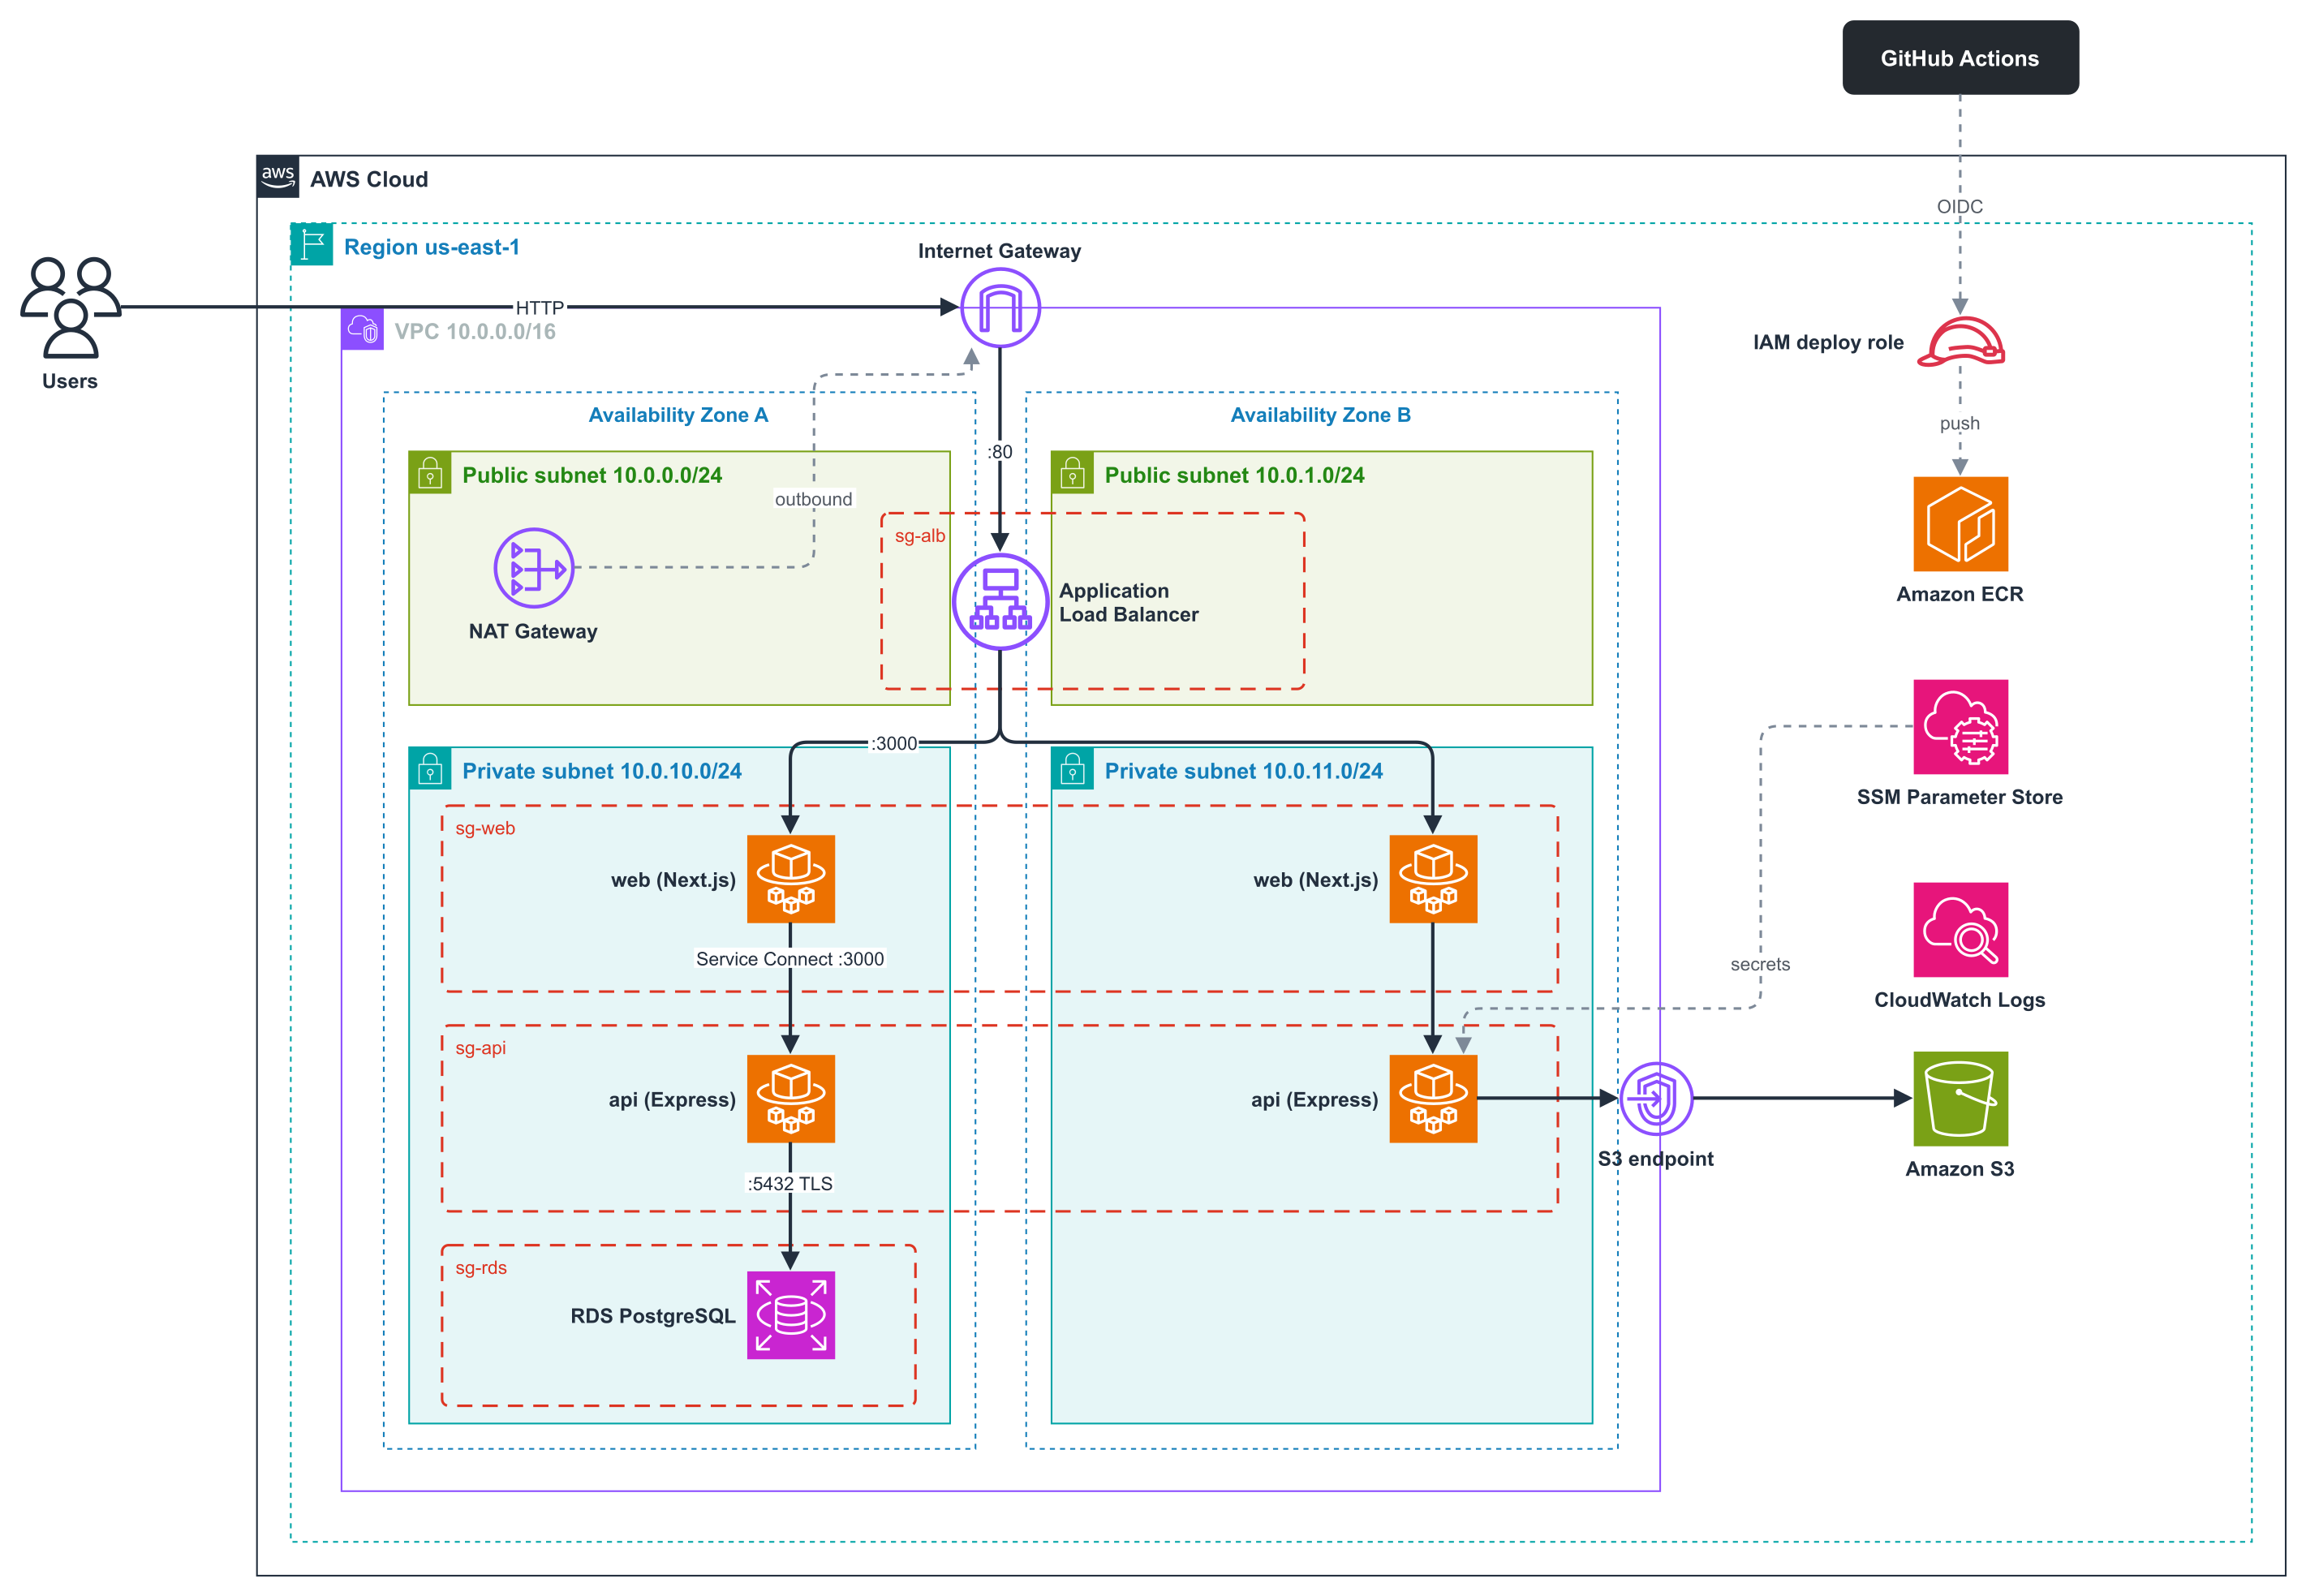
\includegraphics[width=0.93\textwidth]{images/fig_architecture.png}
  \caption{PDF Toolkit on AWS: network design, tiers, security-group boundaries, managed services and the CI/CD flow.}
  \label{fig:arch}
\end{figure}

\textbf{Network.} The VPC \texttt{10.0.0.0/16} spans two Availability Zones
with one public and one private \texttt{/24} subnet in each:
\emph{public} \texttt{10.0.0.0/24}, \texttt{10.0.1.0/24} (ALB and NAT Gateway;
route \texttt{0.0.0.0/0} $\rightarrow$ Internet Gateway) and \emph{private}
\texttt{10.0.10.0/24}, \texttt{10.0.11.0/24} (all containers and RDS; route
$\rightarrow$ NAT Gateway, outbound only). A free S3 gateway endpoint on the
private route table keeps file traffic inside AWS and off the NAT.

\textbf{Request flow.} Browser $\rightarrow$ internet-facing ALB (:80)
$\rightarrow$ web task (Next.js :3000) $\rightarrow$ \texttt{/api/*} rewritten
to \texttt{http://api:3000} and resolved by \emph{ECS Service Connect}
$\rightarrow$ API task (Express :3000) $\rightarrow$ RDS (:5432, TLS with
certificate verification) and S3 (HTTPS via the gateway endpoint).

\textbf{Key decisions.}
\begin{itemize}
  \item \emph{Two separate ECS services:} the tiers scale and fail
        independently and each has its own security group; the API is not
        registered with the ALB, so it is reachable only from the web tier.
  \item \emph{ECS Fargate instead of EC2 ASGs or EKS:} no hosts, AMIs or
        control-plane fee; ECS Service Auto Scaling is the horizontal-scaling
        equivalent of an ASG. The images are standard OCI images, so moving to
        EC2 or Kubernetes needs no application change.
  \item \emph{Service Connect instead of an internal ALB:} a stable name
        (\texttt{api}) with client-side load balancing, at no extra cost.
  \item \emph{Stateless containers:} identity is a JWT cookie and all state
        lives in RDS (metadata) or S3 (PDF bytes), so any task can serve any
        request. Migrations run at start-up under a PostgreSQL advisory lock.
\end{itemize}

% =============================================================================
\section{Services Used and Their Role in Each Tier}
% =============================================================================
\begin{table}[H]
\centering\footnotesize
\begin{tabularx}{\textwidth}{L{2.3cm}L{6.6cm}X}
\toprule
\textbf{Tier / concern} & \textbf{AWS service (configuration)} & \textbf{Role}\\
\midrule
Network & VPC, 4 subnets in 2 AZs, IGW, 1 NAT Gateway, 2 route tables, S3 gateway endpoint & Segmentation, controlled connectivity\\
Entry / LB & Internet-facing ALB, IP target group \texttt{web} (health check \texttt{/}), listener :80 & Single public endpoint, distributes requests\\
Web tier & ECS Fargate service \texttt{web}, 0.25 vCPU / 0.5\,GB, 1--2 tasks & Next.js container: UI, proxies \texttt{/api/*}\\
Application tier & ECS Fargate service \texttt{api}, 0.25 vCPU / 0.5\,GB, 1--2 tasks, Service Connect & Express container: auth, PDF processing, history\\
Database tier & RDS PostgreSQL 16.15, db.t4g.micro, gp3 20\,GB, encrypted, not public & Users and document metadata, backups, patching\\
Object storage & S3 bucket: public access blocked, TLS-only policy, \texttt{tmp/} expiry 1 day & Uploaded and generated PDFs\\
Registry & Amazon ECR, 2 repositories, scan on push, keep last 10 & Images tagged \texttt{latest} and commit SHA\\
Secrets / identity & SSM Parameter Store (SecureString); IAM execution, task and GitHub OIDC roles & DB URL and JWT secret; least privilege, keyless CI\\
Observability & CloudWatch Logs (\texttt{awslogs}, 7-day retention), ECS metrics & Centralised logs, scaling metric\\
\bottomrule
\end{tabularx}
\caption{Services and their roles. All 64 resources are provisioned by Terraform.}
\end{table}

% =============================================================================
\section{Containerization and CI/CD Pipeline Design}
% =============================================================================
\textbf{Containers.} Both images use multi-stage \texttt{node:20-alpine}
Dockerfiles, are built from the monorepo root and run as the non-root
\texttt{node} user on port 3000 with a container health check.
\begin{itemize}
  \item \emph{Web:} Next.js \texttt{output: "standalone"}; the runtime image
        holds only the standalone server, static assets and \texttt{public/}.
        The API proxy target is a build argument (\texttt{API\_INTERNAL\_URL}).
  \item \emph{API:} installs only its workspace, compiles TypeScript and adds the
        AWS RDS CA bundle so TLS to the database is verified
        (\texttt{verify-full}). All configuration
        comes from environment variables.
  \item \emph{Local orchestration:} \texttt{docker-compose.yml} runs web, API,
        PostgreSQL 16 and MinIO (an S3-compatible stand-in), so the same images
        and code paths run locally and on AWS.
\end{itemize}

\textbf{Pipeline} (\texttt{.github/workflows/ci-cd.yml}):
\begin{enumerate}
  \item \texttt{Build and test} (every push and pull request): \texttt{npm ci},
        type-check both apps, 18 Vitest unit tests, production builds,
        \texttt{terraform fmt -check} and \texttt{terraform validate}.
  \item \texttt{Push images and deploy} (\texttt{main} only, after job 1):
        OIDC login to AWS, Buildx with GitHub layer cache, push
        \texttt{:latest} and \texttt{:<commit-sha>} to ECR, force a new
        deployment of both ECS services, wait until they are stable.
\end{enumerate}
ECS replaces tasks one by one behind the ALB, and the \textbf{deployment
circuit breaker} rolls back automatically if new tasks fail their health
checks. Terraform owns the task definitions, so CI needs no
\texttt{iam:PassRole}. Rollback: set \texttt{image\_tag} to an earlier commit
SHA and \texttt{terraform apply}, or revert the commit.

% =============================================================================
\section{Security Considerations}
% =============================================================================
\begin{table}[H]
\centering\footnotesize
\begin{tabularx}{\textwidth}{L{2.6cm}X}
\toprule
\textbf{Control} & \textbf{Implementation}\\
\midrule
Segmentation & Only the ALB and NAT are in public subnets; no task has a public IP; RDS \texttt{publicly\_accessible = false}.\\
Security groups & Chain of SG references: Internet $\xrightarrow{80}$ alb $\xrightarrow{3000}$ web $\xrightarrow{3000}$ api $\xrightarrow{5432}$ rds. Egress is limited to 443 (AWS APIs) plus the next hop; the RDS SG has no egress.\\
Secrets (app) & Terraform generates the DB password and JWT secret and stores them only as KMS-encrypted SSM SecureStrings. ECS injects them at task start; they never appear in code, images, CI or logs.\\
Secrets (CI/CD) & No AWS keys in GitHub: the workflow exchanges a short-lived OIDC token for the deploy role. The trust policy allows only \texttt{repo:MuhammadTalha57/pdf-toolkit:ref:refs/heads/main}; permissions cover 2 ECR repos and 2 ECS services. Pull requests cannot deploy.\\
IAM & Execution role reads only the 2 parameters; the API task role may only Get/Put/Delete objects in its own bucket; the web task has no AWS permissions.\\
Encryption & TLS to RDS (forced by the server, verified by the client); RDS and S3 encrypted at rest; S3 denies non-TLS requests.\\
Application & bcrypt password hashes, HS256 JWT in an \texttt{httpOnly}, \texttt{SameSite=Lax} cookie, helmet, rate limiting, PDF and UUID validation, per-user ownership checks, ECR vulnerability scanning.\\
\bottomrule
\end{tabularx}
\caption{Security controls.}
\end{table}
\textbf{Verified on the live system:} the RDS endpoint resolves to a private IP
(\texttt{10.0.10.149}) and a TCP connection to 5432 from the internet times
out; \texttt{PubliclyAccessible=False}, \texttt{StorageEncrypted=True};
API requests without a session cookie return \texttt{401}.

% =============================================================================
\section{Cloud-Native Enhancements}
% =============================================================================
\textbf{Object storage (Amazon S3).} Uploads are validated and stored as
\texttt{tmp/<uuid>.pdf}; results go to \texttt{users/<id>/results/<uuid>.pdf}
and the temporary inputs are deleted, with a 1-day lifecycle rule as backstop.
Downloads are streamed by the API after an ownership check, so the bucket
stays private and no presigned URLs are issued.

\textbf{Infrastructure as Code (Terraform).} The whole environment is declared
in \texttt{infra/terraform/} (\texttt{network}, \texttt{security},
\texttt{alb}, \texttt{ecs}, \texttt{rds}, \texttt{s3}, \texttt{ecr},
\texttt{iam}). Variables control sizing and scaling (\texttt{min\_tasks},
\texttt{max\_tasks}, \texttt{db\_multi\_az}, \ldots); every resource carries
default tags. Deployment runs in two phases: the ECR repositories plus a
bootstrap image push, then the remaining 62 resources in about 12 minutes
(RDS 7\,min 42\,s). \texttt{terraform destroy} removes everything.

\textbf{Monitoring (CloudWatch).} The \texttt{awslogs} driver ships both
services' logs to one log group per service (7-day
retention); ECS CPU metrics
drive autoscaling.

\textbf{Cost estimate} (us-east-1, on-demand, 730\,h): Fargate 2 tasks \$18.0,
ALB \$19.4, NAT \$33.1, public IPv4 \$11.0, RDS + storage \$14.0, S3/ECR/logs/
transfer \$1.9 $\Rightarrow$ \textbf{$\approx$ \$97/month} ($\approx$\$3.20/day;
$\approx$\$115 at full scale). Optimisations: (1)~one NAT instead of one per
AZ, with the free S3 endpoint keeping PDF traffic off it ($\approx$\$37/month
saved); (2)~1-task baseline that scales to 2 only under load, at the smallest
Fargate size ($\approx$\$18/month saved); (3)~lifecycle rules, 7-day logs and
one-command teardown. Further options: Graviton (ARM64) tasks ($\approx$20\,\%
off Fargate), Fargate Spot, Savings Plans.

% =============================================================================
\section{Testing Results: Successful Automated Deployment}
% =============================================================================
\begin{table}[H]
\centering\footnotesize
\begin{tabularx}{\textwidth}{L{6.4cm}X}
\toprule
\textbf{Test} & \textbf{Result}\\
\midrule
Unit tests; type-check; production builds & 18/18 passed (7 suites); both apps pass\\
Local 3-tier stack (Docker Compose) & signup, upload, merge (4 pages), download (\texttt{\%PDF-}) passed\\
\texttt{terraform validate}; \texttt{terraform plan} & valid; 64 resources, no errors\\
\texttt{terraform apply}; target health & 62 added (+2 ECR); web target healthy; both services 1/1 running\\
Smoke test vs.\ public ALB & health ok; signup (RDS), upload (S3), merge, download, 401 without cookie: \textbf{all passed}\\
\textbf{Pipeline run \#2} (commit \texttt{da4c977}) & Build and test 1\,min 39\,s $\rightarrow$ Push images and deploy 8\,min 37\,s; both services rolled out (\texttt{COMPLETED}); total 10\,min 23\,s\\
Image traceability & ECR holds \texttt{latest} and \texttt{da4c9775\ldots} tags pushed by the pipeline\\
\bottomrule
\end{tabularx}
\caption{Test and deployment results (full screenshot set submitted separately in \texttt{screenshots/}).}
\end{table}
\begin{figure}[H]
\centering
\begin{minipage}[t]{0.495\textwidth}\centering
  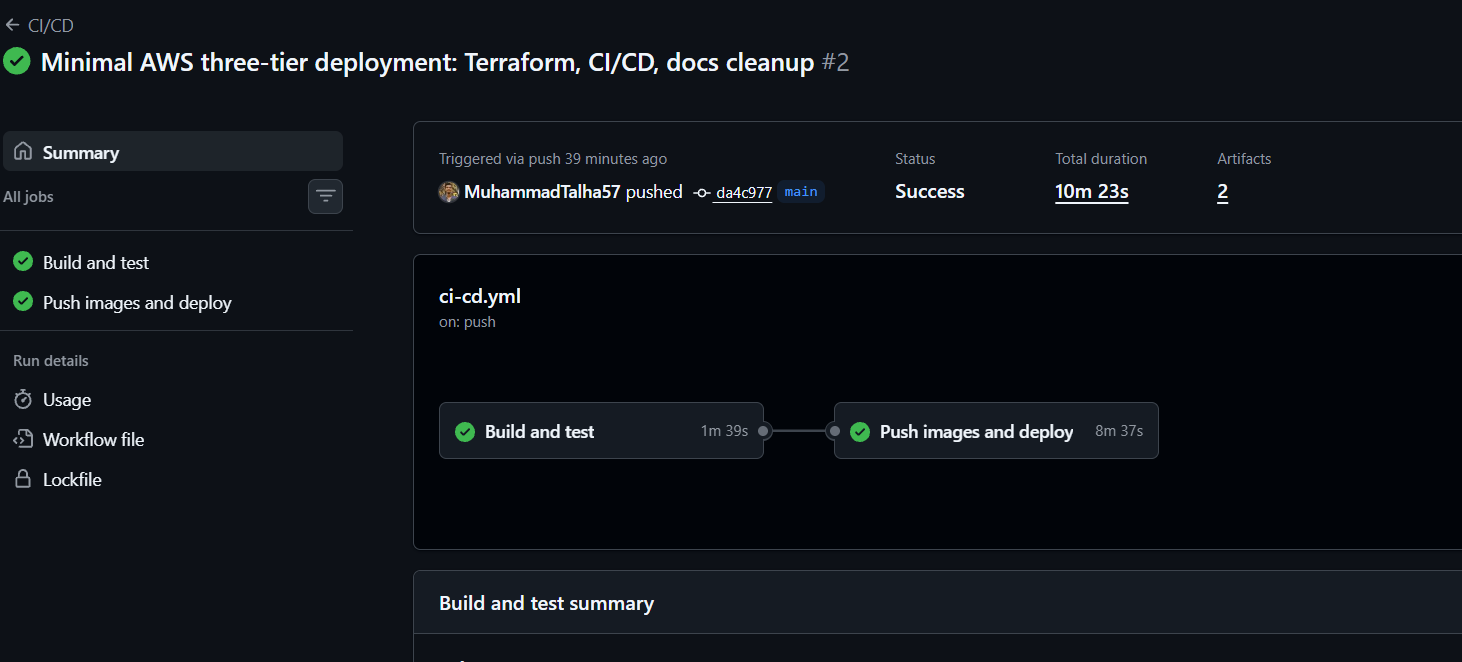
\includegraphics[width=\linewidth]{images/14-github-actions.png}
  \captionof{figure}{Successful pipeline run \#2: both jobs green.}
\end{minipage}\hfill
\begin{minipage}[t]{0.495\textwidth}\centering
  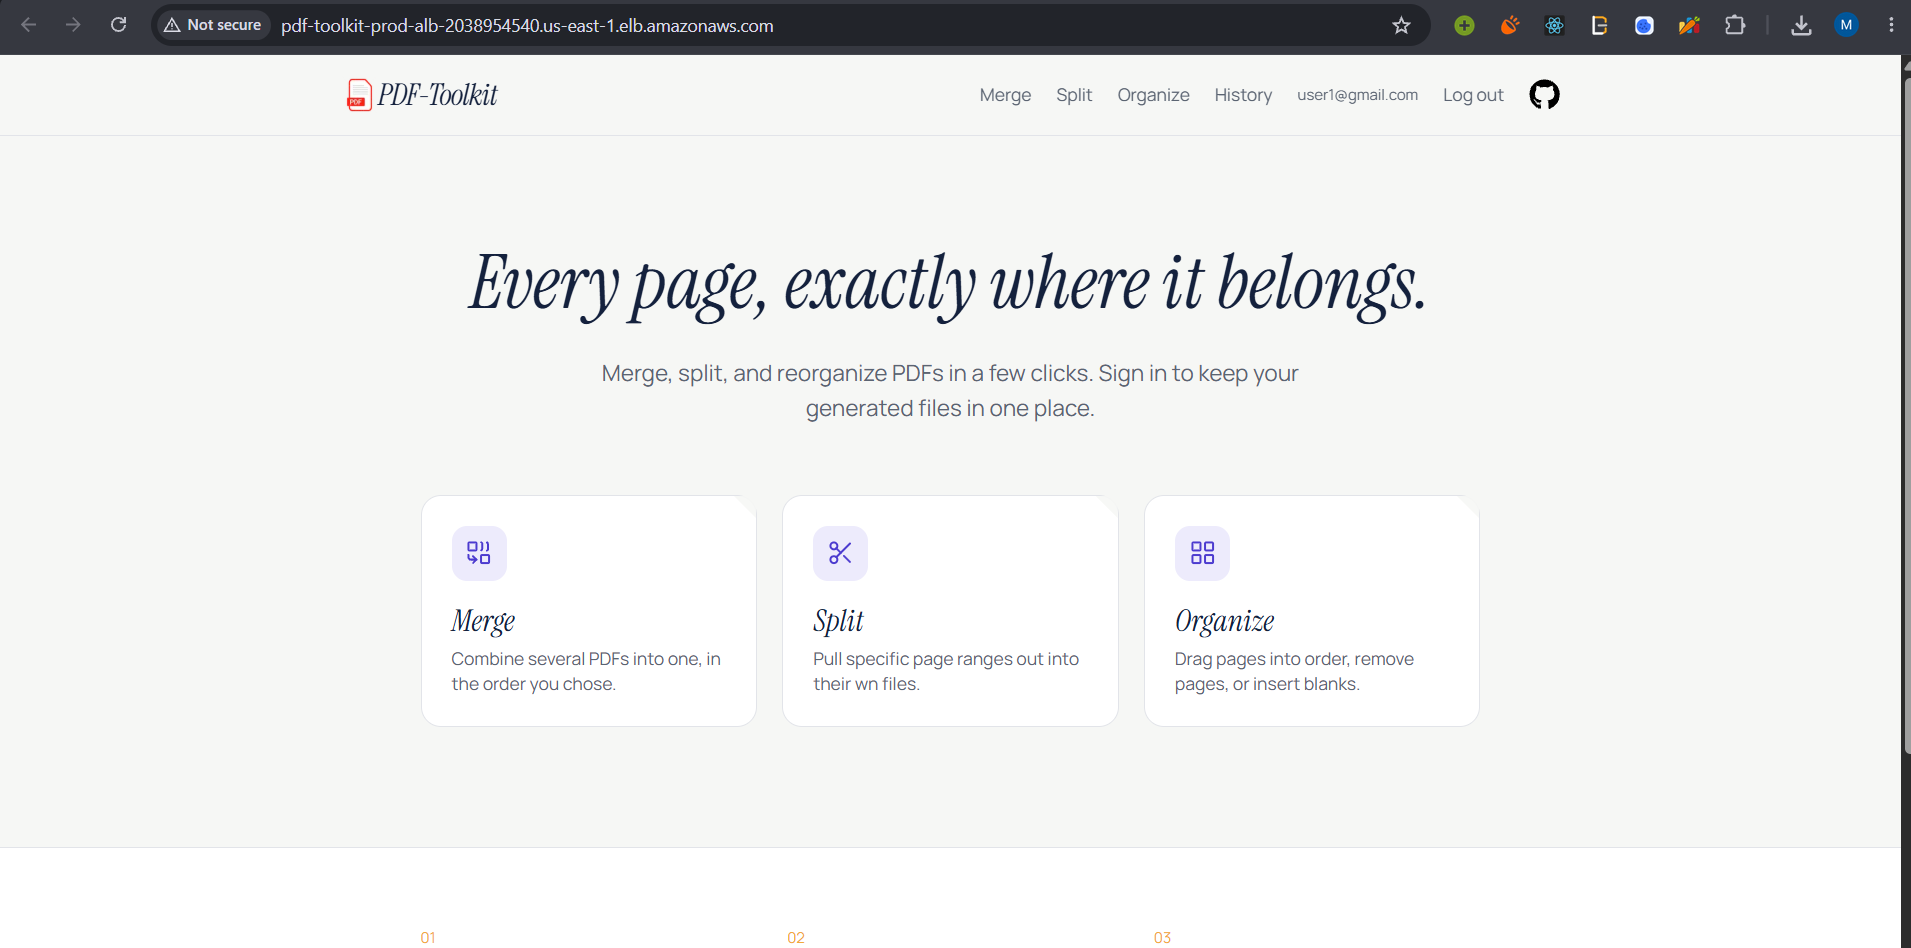
\includegraphics[width=\linewidth]{images/15-app-landing.png}
  \captionof{figure}{The live application at the public ALB URL.}
\end{minipage}\\[3pt]
\begin{minipage}[t]{0.495\textwidth}\centering
  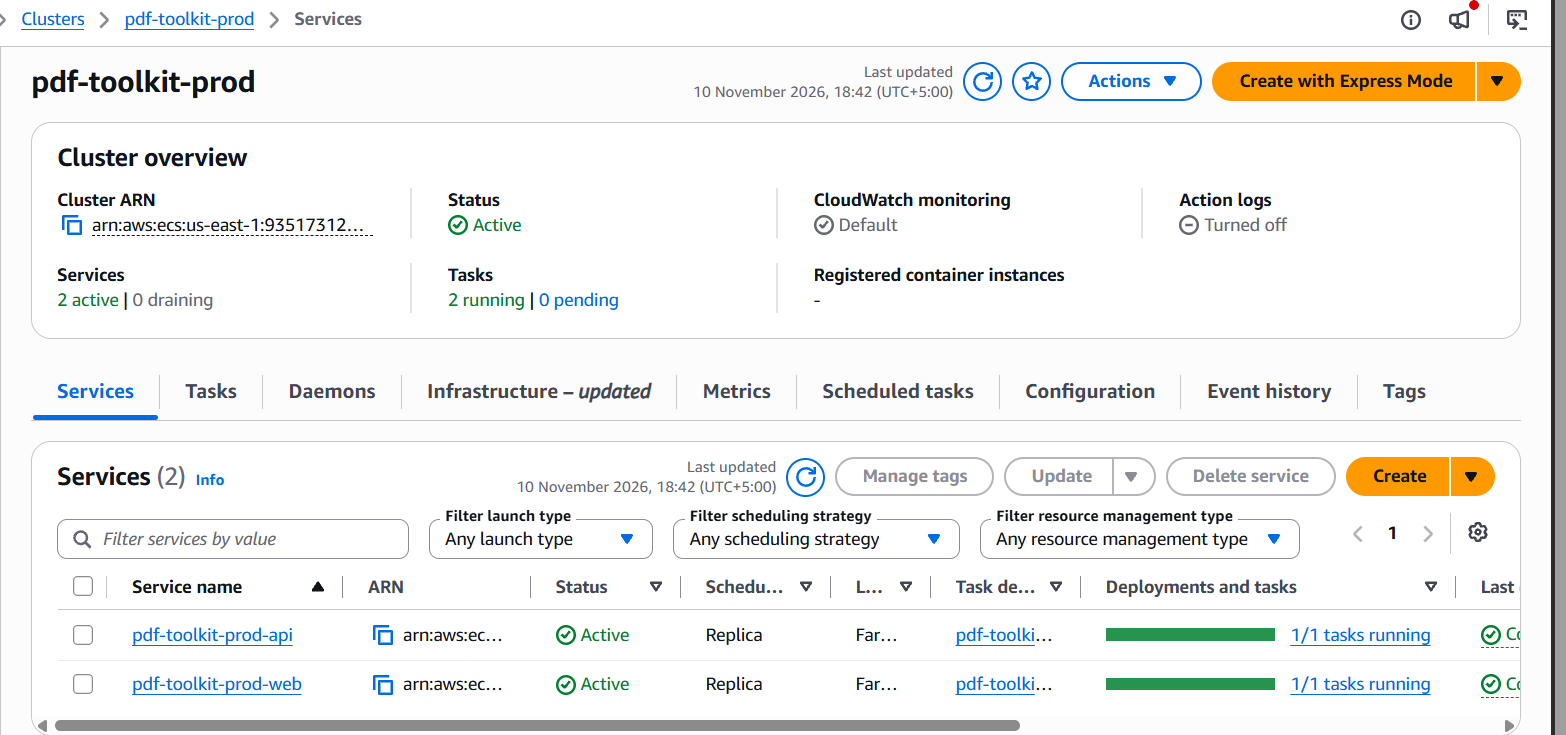
\includegraphics[width=\linewidth]{images/04-ecs-services.png}
  \captionof{figure}{ECS cluster: web and API services, Fargate, 1/1 running.}
\end{minipage}\hfill
\begin{minipage}[t]{0.495\textwidth}\centering
  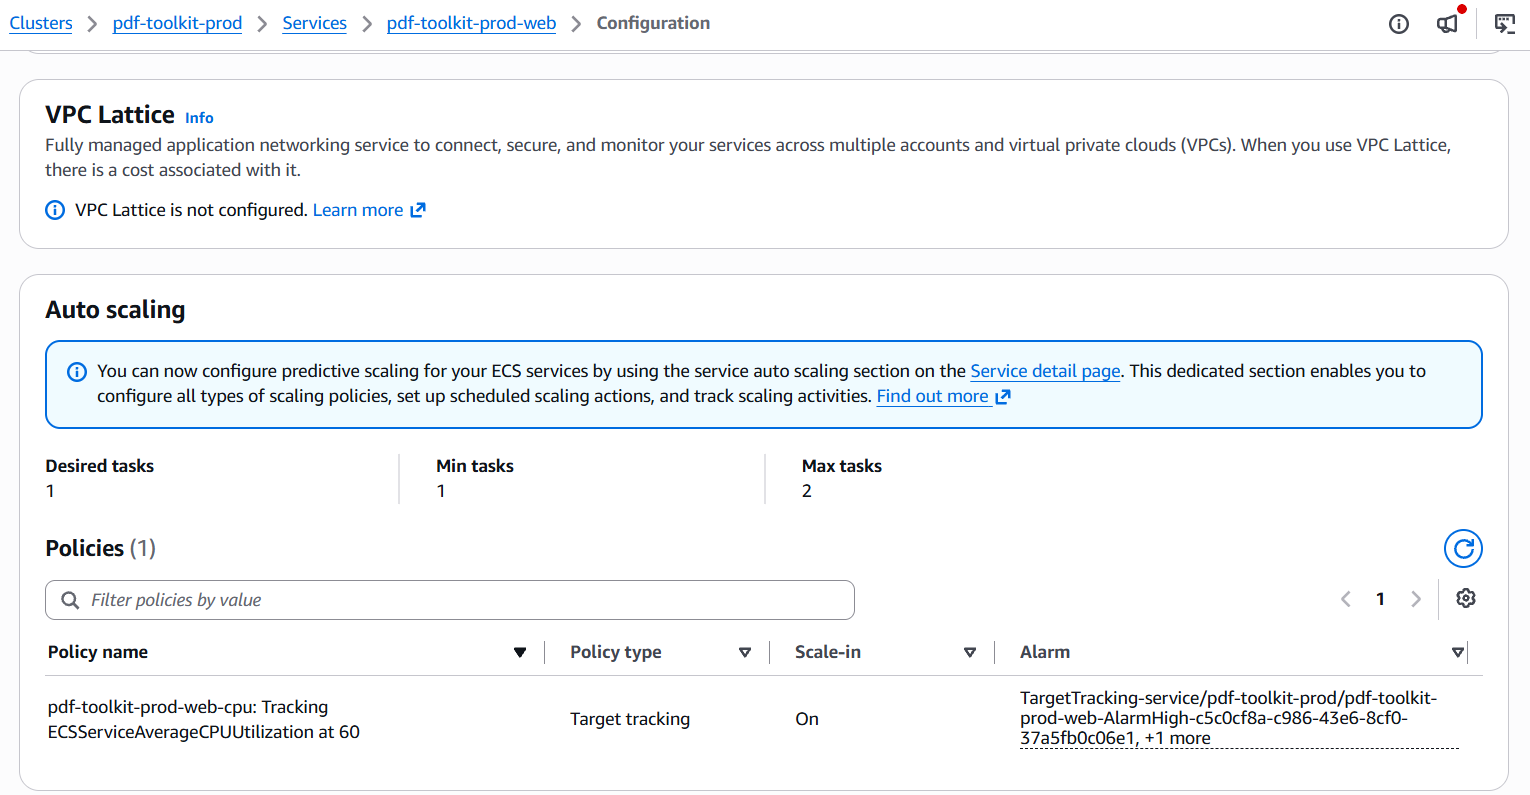
\includegraphics[width=\linewidth]{images/10-autoscaling.png}
  \captionof{figure}{Service auto scaling: min 1, max 2, target 60\,\% CPU.}
\end{minipage}\\[3pt]
\begin{minipage}[t]{0.495\textwidth}\centering
  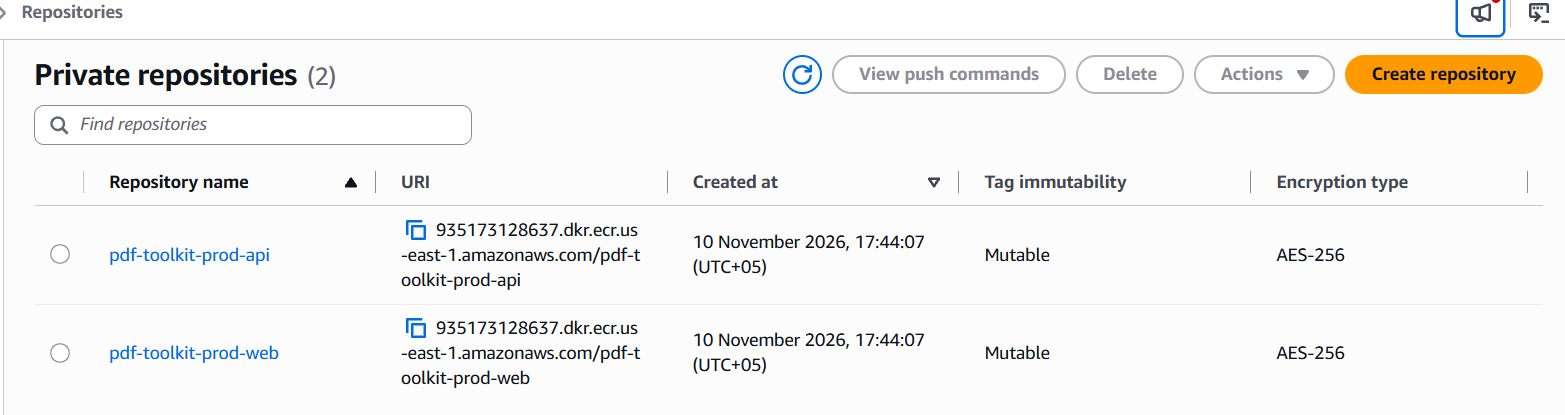
\includegraphics[width=\linewidth]{images/13-ecr-images.png}
  \captionof{figure}{ECR: images pushed by the pipeline (\texttt{latest} + commit SHA).}
\end{minipage}\hfill
\begin{minipage}[t]{0.495\textwidth}\centering
  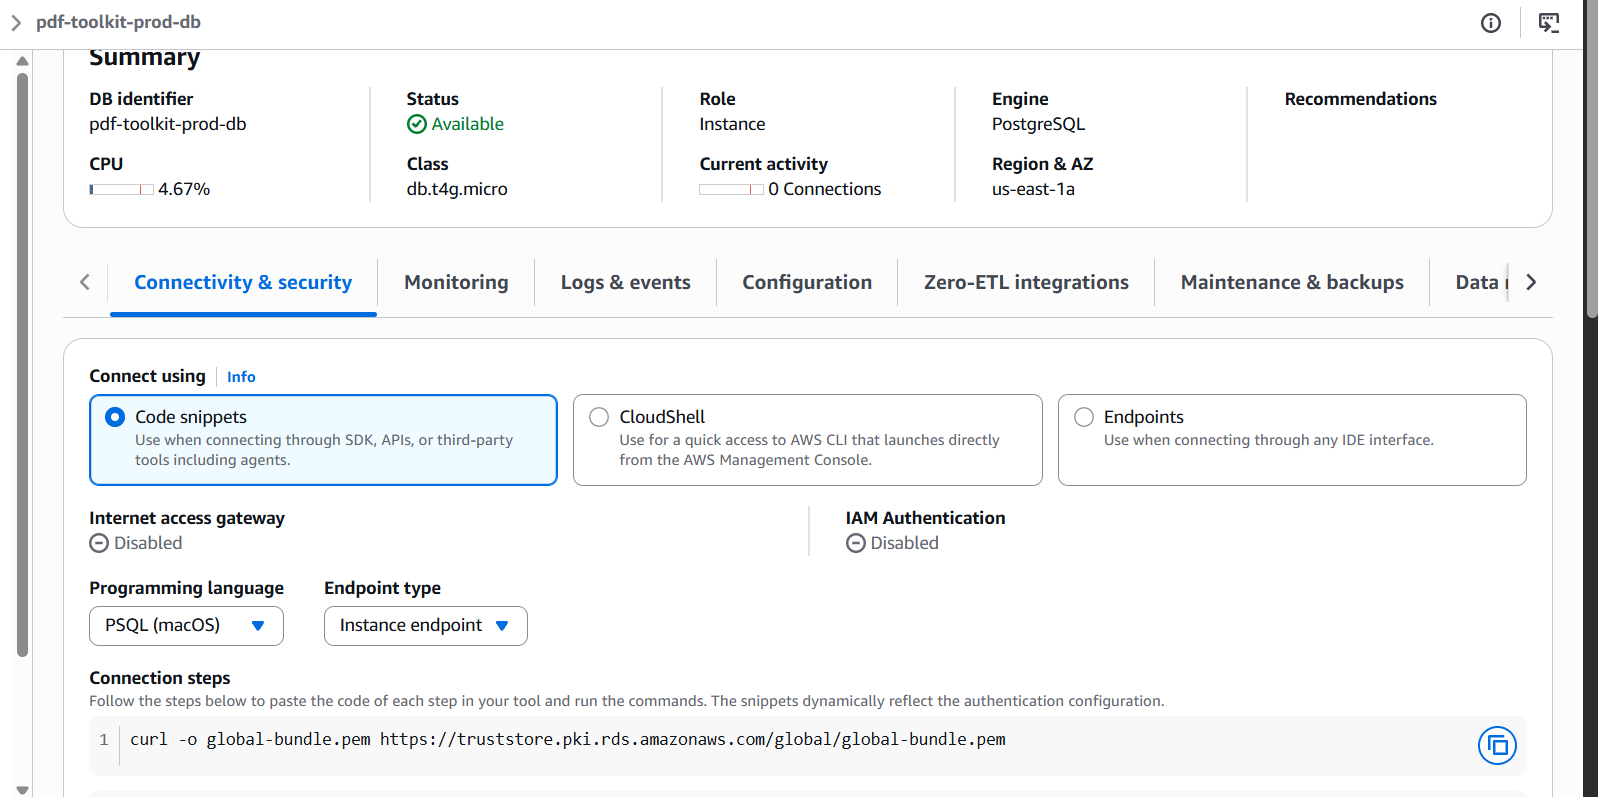
\includegraphics[width=\linewidth]{images/11-rds.png}
  \captionof{figure}{RDS PostgreSQL (db.t4g.micro), no internet access gateway.}
\end{minipage}
\end{figure}

\textbf{Problems solved during deployment.}
\begin{itemize}
  \item \emph{ECS cannot start without an image:} two-phase apply (ECR
        repositories, bootstrap push with the push-images script, then
        the rest).
  \item \emph{\texttt{docker login} to ECR returned \texttt{400 Bad Request}:}
        the CLI's default region (\texttt{ap-south-1}) differed from the
        registry's; the scripts now derive the region from the registry host.
  \item \emph{OIDC subject mismatch:} running the deploy job in a GitHub
        \emph{environment} changes the token subject to
        \texttt{:environment:\ldots}, which the main-branch-only trust policy
        rejects; the job runs without an environment.
  \item \emph{Terraform vs.\ autoscaler:} \texttt{desired\_count} is ignored
        after creation so \texttt{apply} never undoes a scale-out.
\end{itemize}

% =============================================================================
\section{Non-Functional Requirements (NFR) Justification}
% =============================================================================
\begin{table}[H]
\centering\footnotesize
\begin{tabularx}{\textwidth}{L{2.05cm}L{8.1cm}X}
\toprule
\textbf{NFR} & \textbf{Design / implementation decisions} & \textbf{Limitations $\rightarrow$ improvement}\\
\midrule
Scalability & Stateless containers scale horizontally; ALB (web) and Service Connect (API) distribute load; tiers scale independently; S3 has no capacity limit; indexed queries. & Single DB writer; demo cap of 2 tasks $\rightarrow$ read replicas, RDS Proxy, higher \texttt{max\_tasks}.\\
Availability & 2 AZs; ALB and container health checks replace failed tasks; circuit breaker rolls back bad releases; RDS automated backups; S3 is multi-AZ. & 1-task minimum, one NAT and Single-AZ RDS $\rightarrow$ \texttt{min\_tasks = 2}, per-AZ NAT, \texttt{db\_multi\_az = true}.\\
Elasticity & Target tracking at 60\,\% CPU adds a task after 60\,s above target and removes it after a 300\,s cooldown; nothing is sized for peak. & Not load-tested; CPU is the only signal $\rightarrow$ request-count or scheduled scaling.\\
Security & Segmentation, chained SGs, least-privilege IAM, SSM secrets, OIDC CI, verified TLS to RDS, encryption at rest, non-root containers; verified live. & HTTP only (no domain), no WAF, secrets in local TF state $\rightarrow$ ACM + HTTPS, WAF, encrypted remote state.\\
Maintain-\newline ability / Deploy-\newline ability & Everything in Terraform; every push tested and every \texttt{main} commit deployed automatically; rolling updates with auto-rollback; SHA-tagged images; same images locally and on AWS. & No staging environment $\rightarrow$ Terraform workspaces and an approval gate.\\
Performance & Web and API scale separately so PDF work cannot starve the UI; client-side previews (pdf.js) avoid round-trips; streamed downloads; S3 via gateway endpoint. & 0.25 vCPU tasks; far region for users in Pakistan; no CDN $\rightarrow$ larger tasks, \texttt{ap-south-1}, CloudFront, SQS workers.\\
Cost-efficiency & Smallest sizes, 1-task baseline, single NAT, free S3 endpoint, lifecycle rules, 7-day logs, one-command destroy ($\approx$\$97/month). & NAT, ALB and IPv4 are fixed (65\,\%) $\rightarrow$ Graviton, Spot, Savings Plans.\\
Portability & OCI images configured by environment variables run unchanged under Compose, ECS or Kubernetes; S3 API (works with MinIO); plain PostgreSQL. & IaC uses AWS-specific services $\rightarrow$ Kubernetes/Helm for the app layer.\\
\bottomrule
\end{tabularx}
\caption{Mapping of design decisions to NFRs, including known limitations.}
\end{table}

% =============================================================================
\section{Conclusion and Deliverables}
% =============================================================================
PDF Toolkit runs on AWS as a segmented, load-balanced, auto-scaling three-tier
system with a private, TLS-enforced managed database and private object
storage. Every push to \texttt{main} is tested, built, pushed to ECR and rolled
out automatically without any long-lived credentials, and the entire
environment is reproducible from Terraform. The main open items --- HTTPS, a
Multi-AZ database and NAT, and a higher task minimum --- are configuration-level
changes.

\textbf{Deliverables.}
\begin{itemize}
  \item Architecture diagram: Figure~\ref{fig:arch} (\texttt{01-architecture-diagram/}).
  \item Screenshots: \texttt{02-screenshots/}.
  \item Source files (\texttt{03-source-files/}): web and API Dockerfiles,
        \texttt{docker-compose.yml}, the GitHub Actions workflow and the
        Terraform configuration.
  \item Repository: \url{\repourl}
  \item Live application: {\small\url{\appurl}}
  \item Kubernetes manifests: not applicable (ECS Fargate).
\end{itemize}

\end{document}
